\documentclass{beamer}
\usepackage{graphics}

% Beamer appearance
\usepackage{helvet}
\definecolor{MaltaBlue}{RGB}{81,118,147}
\definecolor{FireBrick}{RGB}{228,34,23}
\setbeamertemplate{navigation symbols}{}
\setbeamertemplate{headline}{} % removes navtree
\setbeamercolor{example text}{fg=black}
\setbeamercolor{footline}{fg=black}
\setbeamercolor{structure}{fg=black}
\setbeamercolor{alerted text}{fg=FireBrick}
\setbeamertemplate{footline}{\strut\hfill%
\insertframenumber~~}%/\inserttotalframenumber~~}

\renewcommand{\baselinestretch}{1.5}

\title{Artisanal Type Theory}
\author{Carlo Angiuli}
\date{April 1, 2015}
\institute{Carnegie Mellon University}

\usebackgroundtemplate%
{
\includegraphics[width=\paperwidth,height=\paperheight]{bg.jpg}}

\begin{document}

\begin{frame}
\maketitle
\end{frame}

\begin{frame}
\centering
{\LARGE Computers have ruined good, old-fashioned computing.}
\end{frame}

% Back in the day, computing was hard.
\begin{frame}
\centering
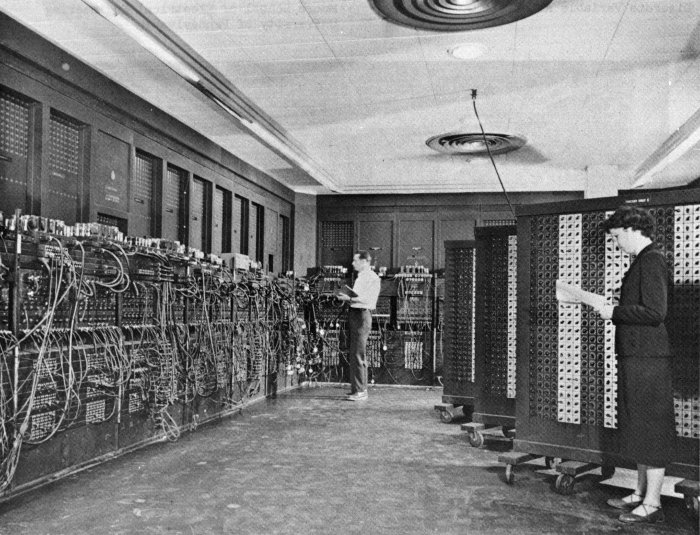
\includegraphics[width=4in]{eniac.jpg}
\end{frame}

% No, I mean earlier than that.
\begin{frame}
\centering
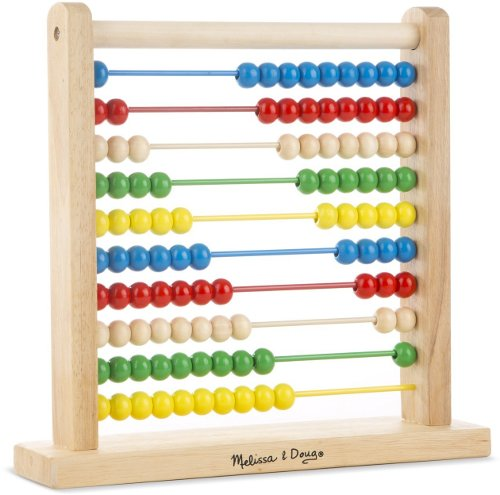
\includegraphics[width=3.25in]{abacus.jpg}
\end{frame}

% It was the domain of skilled craftspeople, just like food was.
\begin{frame}
\centering
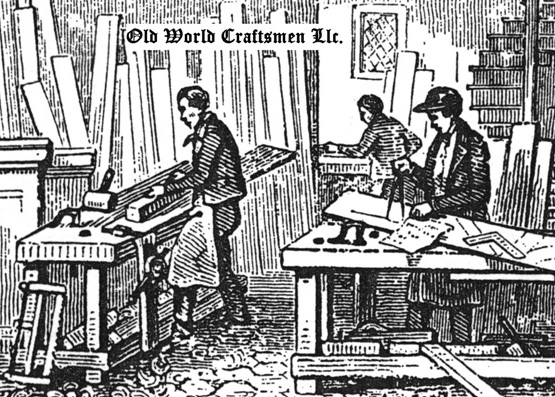
\includegraphics[width=4in]{craftsmen.jpg}
\end{frame}

% But now food is made by the ton in heartless factories.
\begin{frame}
\centering
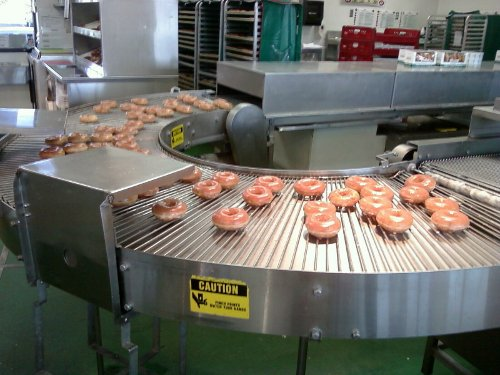
\includegraphics[width=4in]{donut.jpg}
\end{frame}

% The artisanal food movement has reclaimed food...
\begin{frame}
\centering
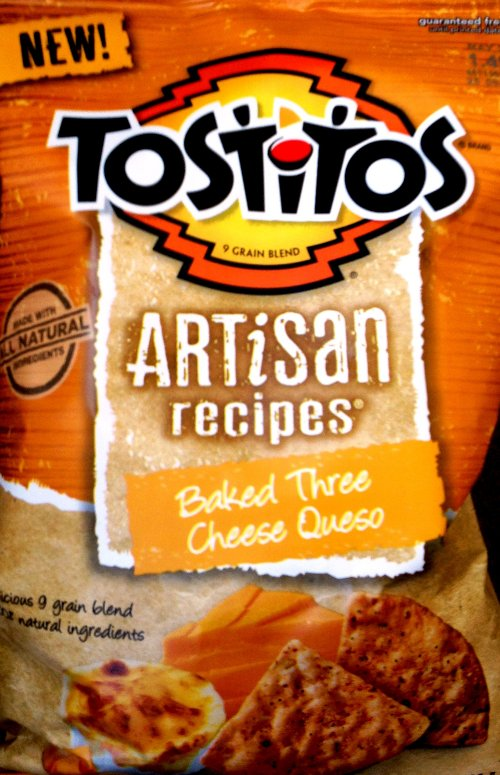
\includegraphics[width=2in]{tostitos.jpg}
\end{frame}

% ...and some mechanical tasks.
\begin{frame}
\centering
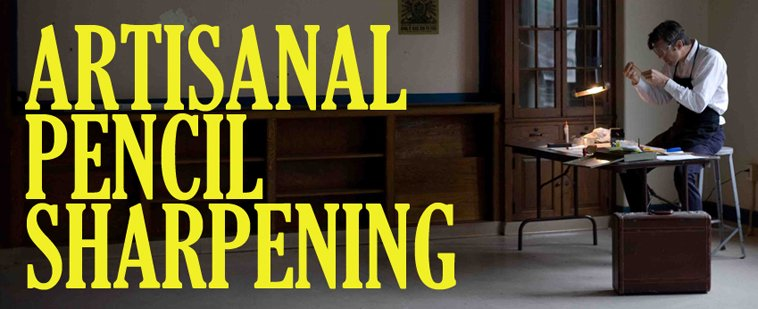
\includegraphics[width=4in]{pencil.jpg}
\end{frame}

% Computers have replaced the human aspect of computation.
\begin{frame}
\centering
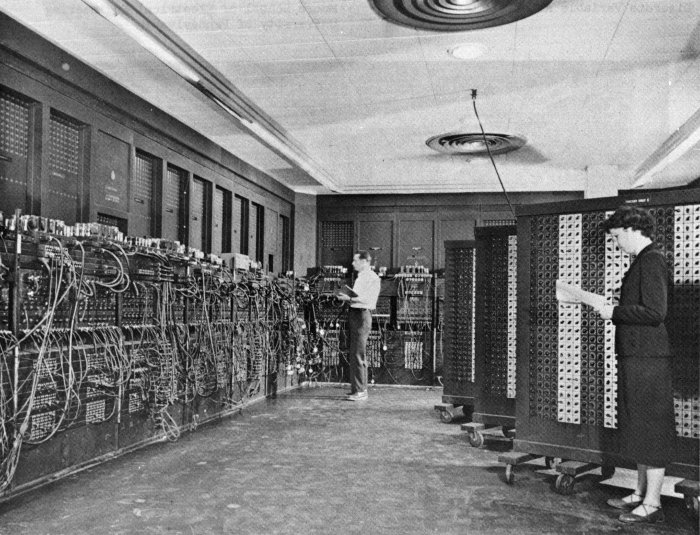
\includegraphics[width=4in]{eniac.jpg}
\end{frame}


% Even computer programs themselves are churned out day-in, day-out
\begin{frame}
\centering
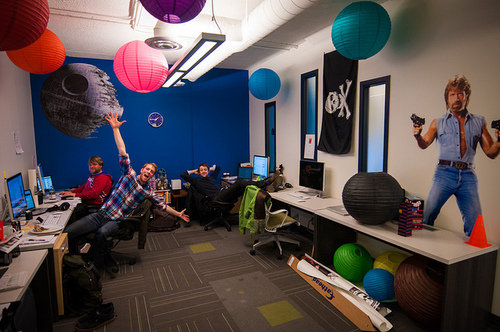
\includegraphics[width=4in]{startup.jpg}
\end{frame}

% in heartless factories.
\begin{frame}
\centering

\includegraphics[width=3in]{ycomb.png}
\end{frame}

\begin{frame}
\centering
{\LARGE Artisanal Type Theory: \\ A more \emph{personal} \\
foundation for computation}
\end{frame}

\begin{frame}
\Large
Deduction with a commitment to locally-
\begin{itemize}
\Large
\item grown,
\item sound, and
\item complete reasoning.
\end{itemize}
\end{frame}

\begin{frame}
\centering
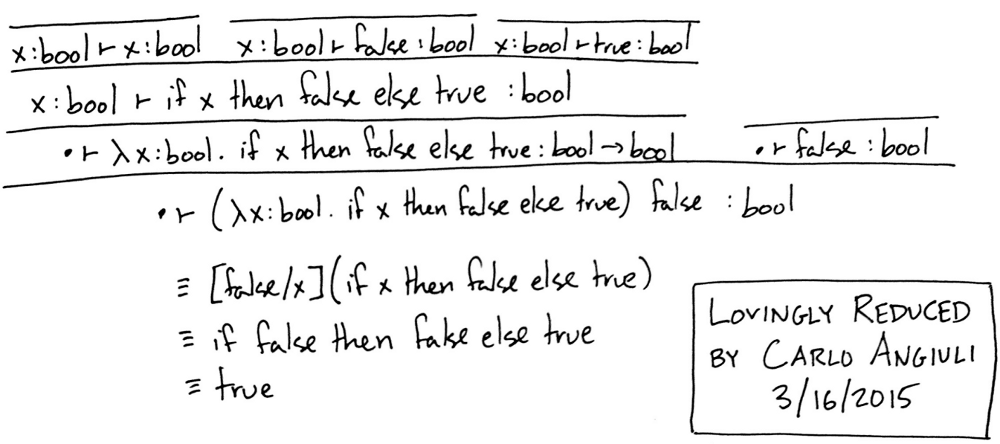
\includegraphics[width=4.3in]{../isfalse.png}
\end{frame}

\begin{frame}
\Large
Applications to
\begin{itemize}
\Large
\item Shallow learning
\item Fairly quick sorting
\item Small-batch jobs
\end{itemize}
\end{frame}

\begin{frame}
\centering
\LARGE
See the SIGBOVIK 2015 proceedings!
\end{frame}

\end{document}

